\tikzset{every picture/.style={line width=0.75pt}} %set default line width to 0.75pt        

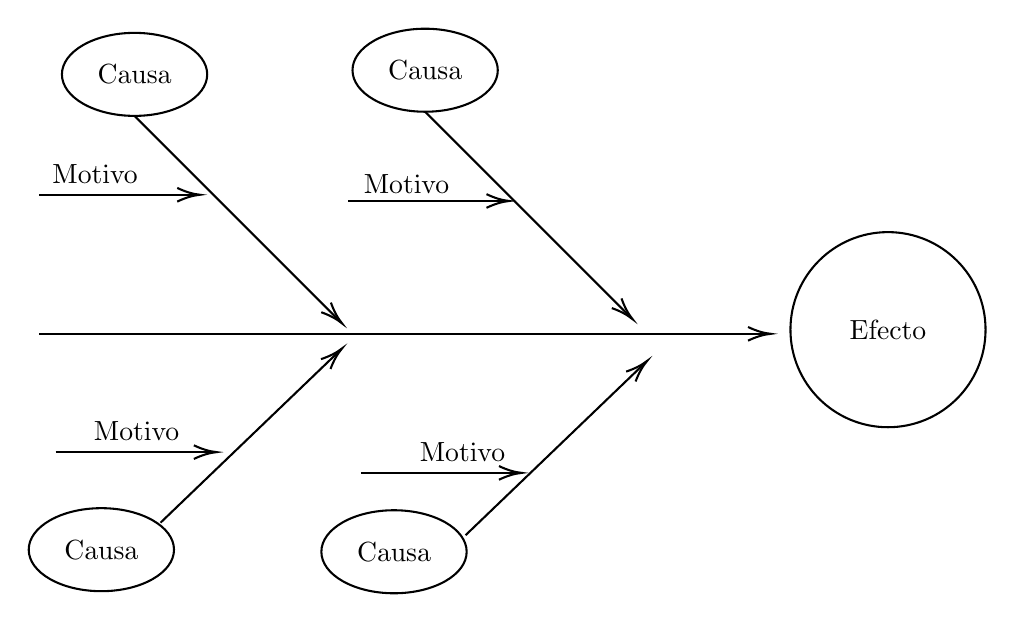
\begin{tikzpicture}[x=0.75pt,y=0.75pt,yscale=-1,xscale=1]
%uncomment if require: \path (0,300); %set diagram left start at 0, and has height of 300

%Shape: Circle [id:dp5990397926815021] 
\draw   (444,172) .. controls (444,146.04) and (465.04,125) .. (491,125) .. controls (516.96,125) and (538,146.04) .. (538,172) .. controls (538,197.96) and (516.96,219) .. (491,219) .. controls (465.04,219) and (444,197.96) .. (444,172) -- cycle ;
%Straight Lines [id:da4633423943796984] 
\draw    (82,174) -- (432.5,174) ;
\draw [shift={(434.5,174)}, rotate = 180] [color={rgb, 255:red, 0; green, 0; blue, 0 }  ][line width=0.75]    (10.93,-3.29) .. controls (6.95,-1.4) and (3.31,-0.3) .. (0,0) .. controls (3.31,0.3) and (6.95,1.4) .. (10.93,3.29)   ;

%Straight Lines [id:da558271838087038] 
\draw    (128,69) -- (226.59,167.59) ;
\draw [shift={(228,169)}, rotate = 225] [color={rgb, 255:red, 0; green, 0; blue, 0 }  ][line width=0.75]    (10.93,-3.29) .. controls (6.95,-1.4) and (3.31,-0.3) .. (0,0) .. controls (3.31,0.3) and (6.95,1.4) .. (10.93,3.29)   ;

%Straight Lines [id:da23037397947330063] 
\draw    (140.5,265) -- (226.56,182.39) ;
\draw [shift={(228,181)}, rotate = 496.17] [color={rgb, 255:red, 0; green, 0; blue, 0 }  ][line width=0.75]    (10.93,-3.29) .. controls (6.95,-1.4) and (3.31,-0.3) .. (0,0) .. controls (3.31,0.3) and (6.95,1.4) .. (10.93,3.29)   ;

%Straight Lines [id:da43198867902129967] 
\draw    (287.5,271) -- (373.56,188.39) ;
\draw [shift={(375,187)}, rotate = 496.17] [color={rgb, 255:red, 0; green, 0; blue, 0 }  ][line width=0.75]    (10.93,-3.29) .. controls (6.95,-1.4) and (3.31,-0.3) .. (0,0) .. controls (3.31,0.3) and (6.95,1.4) .. (10.93,3.29)   ;

%Straight Lines [id:da9068198028720342] 
\draw    (268,67) -- (366.59,165.59) ;
\draw [shift={(368,167)}, rotate = 225] [color={rgb, 255:red, 0; green, 0; blue, 0 }  ][line width=0.75]    (10.93,-3.29) .. controls (6.95,-1.4) and (3.31,-0.3) .. (0,0) .. controls (3.31,0.3) and (6.95,1.4) .. (10.93,3.29)   ;

%Shape: Ellipse [id:dp2821026210875348] 
\draw   (93,49) .. controls (93,37.95) and (108.67,29) .. (128,29) .. controls (147.33,29) and (163,37.95) .. (163,49) .. controls (163,60.05) and (147.33,69) .. (128,69) .. controls (108.67,69) and (93,60.05) .. (93,49) -- cycle ;
%Shape: Ellipse [id:dp4112338677098557] 
\draw   (233,47) .. controls (233,35.95) and (248.67,27) .. (268,27) .. controls (287.33,27) and (303,35.95) .. (303,47) .. controls (303,58.05) and (287.33,67) .. (268,67) .. controls (248.67,67) and (233,58.05) .. (233,47) -- cycle ;
%Shape: Ellipse [id:dp03926576767494727] 
\draw   (77,278) .. controls (77,266.95) and (92.67,258) .. (112,258) .. controls (131.33,258) and (147,266.95) .. (147,278) .. controls (147,289.05) and (131.33,298) .. (112,298) .. controls (92.67,298) and (77,289.05) .. (77,278) -- cycle ;
%Shape: Ellipse [id:dp1952188134422188] 
\draw   (218,279) .. controls (218,267.95) and (233.67,259) .. (253,259) .. controls (272.33,259) and (288,267.95) .. (288,279) .. controls (288,290.05) and (272.33,299) .. (253,299) .. controls (233.67,299) and (218,290.05) .. (218,279) -- cycle ;
%Straight Lines [id:da7085896023353757] 
\draw    (82,107) -- (157.5,107) ;
\draw [shift={(159.5,107)}, rotate = 180] [color={rgb, 255:red, 0; green, 0; blue, 0 }  ][line width=0.75]    (10.93,-3.29) .. controls (6.95,-1.4) and (3.31,-0.3) .. (0,0) .. controls (3.31,0.3) and (6.95,1.4) .. (10.93,3.29)   ;

%Straight Lines [id:da15649090036211555] 
\draw    (231,110) -- (306.5,110) ;
\draw [shift={(308.5,110)}, rotate = 180] [color={rgb, 255:red, 0; green, 0; blue, 0 }  ][line width=0.75]    (10.93,-3.29) .. controls (6.95,-1.4) and (3.31,-0.3) .. (0,0) .. controls (3.31,0.3) and (6.95,1.4) .. (10.93,3.29)   ;

%Straight Lines [id:da17262885778102977] 
\draw    (237,241) -- (312.5,241) ;
\draw [shift={(314.5,241)}, rotate = 180] [color={rgb, 255:red, 0; green, 0; blue, 0 }  ][line width=0.75]    (10.93,-3.29) .. controls (6.95,-1.4) and (3.31,-0.3) .. (0,0) .. controls (3.31,0.3) and (6.95,1.4) .. (10.93,3.29)   ;

%Straight Lines [id:da14211058186524306] 
\draw    (90,231) -- (165.5,231) ;
\draw [shift={(167.5,231)}, rotate = 180] [color={rgb, 255:red, 0; green, 0; blue, 0 }  ][line width=0.75]    (10.93,-3.29) .. controls (6.95,-1.4) and (3.31,-0.3) .. (0,0) .. controls (3.31,0.3) and (6.95,1.4) .. (10.93,3.29)   ;


% Text Node
\draw (491,172) node  [align=left] {Efecto};
% Text Node
\draw (128,49) node  [align=left] {Causa};
% Text Node
\draw (268,47) node  [align=left] {Causa};
% Text Node
\draw (112,278) node  [align=left] {Causa};
% Text Node
\draw (253,279) node  [align=left] {Causa};
% Text Node
\draw (109,97) node  [align=left] {Motivo};
% Text Node
\draw (129,221) node  [align=left] {Motivo};
% Text Node
\draw (286,231) node  [align=left] {Motivo};
% Text Node
\draw (259,102) node  [align=left] {Motivo};


\end{tikzpicture}
\begin{center}
